\documentclass[10pt,journal,compsoc]{IEEEtran}

\usepackage{amsmath,amssymb,amsfonts}
\usepackage{graphicx}
\usepackage{tikz}
\usepackage{booktabs}
\usepackage{hyperref}
\usepackage{cite}
\usepackage{microtype}
\usepackage{xcolor}

\usetikzlibrary{shapes,arrows,positioning,calc,decorations.pathmorphing,patterns}

\hypersetup{
    colorlinks=true,
    linkcolor=blue!70!black,
    citecolor=blue!70!black,
    urlcolor=blue!70!black
}

\begin{document}

\title{Phase-1 Engineering Chronicle: Theoretical Foundations, First-Principles Microwave Rationales, and Lumped Circuit Synthesis}

\author{Atharve~Dahima
\thanks{A. Dahima is with the Quantum Hardware and Cryogenic Electronics Research Group. Correspondence: \texttt{atharveeee@gmail.com}. Repository: \url{https://github.com/atharveeee-netizen/7-qubit-superconducting-processor}.}}

\markboth{Quantum Hardware Engineering Laboratory Notes, Phase-1 Report (Theory \& Lumped Synthesis)}%
{Dahima: Phase-1 Engineering Chronicle (Theory \& Lumped Synthesis)}

\maketitle

\begin{abstract}
This engineering chronicle documents the rigorous theoretical foundations and microwave circuit synthesis of a superconducting quantum processor. Operating strictly within the pre-layout phase (Phases 1 and 2), we establish: (1) The physical imperative of non-linear Josephson potential over linear harmonic oscillators; (2) Dilution refrigeration thermal engineering and blackbody photon attenuation; (3) Circuit quantum electrodynamics (cQED) in the dispersive regime ($|\Delta| \gg g$); and (4) The analytical derivation and lumped-element equivalent microwave network synthesis in Ansys Circuit. Crucially, every engineering question---why characteristic impedance is matched to $50\,\Omega$, why specific operating frequencies ($f_q \approx 5.0\text{ GHz}$, $f_r \approx 7.04\text{ GHz}$) are chosen, why exact component values ($C_q = 70\text{ fF}, L_J = 10\text{ nH}, C_r = 340\text{ fF}, L_r = 1.5\text{ nH}, C_c = 4\text{ fF}, C_{\text{in}} = 2\text{ fF}$) are enforced, and why dedicated RF grounding topologies are mandatory---is answered from first principles. An integrated theoretical and microwave lexicon arranged in logical physical sequence concludes this treatise.
\end{abstract}

\begin{IEEEkeywords}
Circuit QED, Transmon Qubit, Josephson Junction, Anharmonicity, Coplanar Waveguide, 50-Ohm Matching, Lumped Synthesis, Ansys Circuit, S-Parameters, Dispersive Readout.
\end{IEEEkeywords}

\section{The Core Theoretical Grounding}

\subsection{Why Superconducting Transmons Over Other Modalities?}
Quantum information processing requires physical systems capable of coherent superposition, high-fidelity gate control, and scalable multi-qubit interconnection. While trapped ions and neutral atoms offer extended coherence times, their gate operation speeds are bounded by optical or acoustic phonon modes ($\mu\text{s}$ to $\text{ms}$ range), and scaling requires complex vacuum-chamber optical routing.

In contrast, superconducting transmons are macroscopic solid-state electrical circuits lithographically patterned onto high-resistivity silicon wafers. They operate at microwave frequencies ($4\text{--}8\text{ GHz}$), allowing coherent gate manipulation via standard RF microwave equipment with pulse durations on the order of $10\text{--}30\text{ ns}$. Most crucially, they are designed, optimized, and verified using established electromagnetic Electronic Design Automation (EDA) frameworks (Ansys HFSS, Q3D, Qiskit Metal).

\begin{figure}[!ht]
\centering
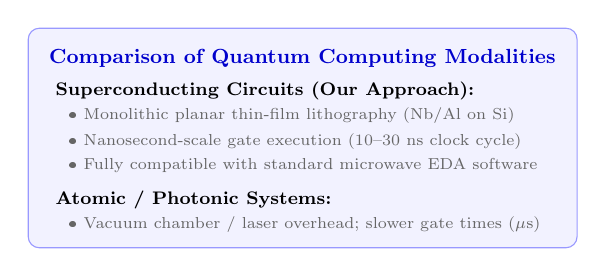
\begin{tikzpicture}[scale=0.82, every node/.style={transform shape}]
    \draw[fill=blue!5, draw=blue!40, rounded corners=4pt] (0,0) rectangle (8.5, 3.4);
    \node[anchor=north west, font=\bfseries\small, text=blue!80!black] at (0.2, 3.2) {Comparison of Quantum Computing Modalities};
    \node[anchor=north west, font=\footnotesize] at (0.3, 2.7) {\textbf{Superconducting Circuits (Our Approach):}};
    \node[anchor=north west, font=\scriptsize, text=gray!80!black] at (0.5, 2.3) {• Monolithic planar thin-film lithography (Nb/Al on Si)};
    \node[anchor=north west, font=\scriptsize, text=gray!80!black] at (0.5, 1.9) {• Nanosecond-scale gate execution (10--30 ns clock cycle)};
    \node[anchor=north west, font=\scriptsize, text=gray!80!black] at (0.5, 1.5) {• Fully compatible with standard microwave EDA software};
    \node[anchor=north west, font=\footnotesize] at (0.3, 1.0) {\textbf{Atomic / Photonic Systems:}};
    \node[anchor=north west, font=\scriptsize, text=gray!80!black] at (0.5, 0.6) {• Vacuum chamber / laser overhead; slower gate times ($\mu$s)};
\end{tikzpicture}
\caption{Architectural advantages of superconducting circuit QED.}
\label{fig:modalities}
\end{figure}

\subsection{Cryogenic Thermal Engineering: The Dilution Refrigerator}

\subsubsection{Why Must the Processor Operate at 10 to 15 mK?}
At room temperature ($T = 300\text{ K}$), the thermal energy $k_B T \approx 25.8\text{ meV}$ dwarfs the energy of a single microwave photon:
\begin{equation}
E_{\text{photon}} = \hbar \omega_{01} \approx h \times (5.0\text{ GHz}) \approx 20.7\,\mu\text{eV}
\end{equation}
Thermal blackbody fluctuations at $300\text{ K}$ would immediately randomize the qubit state via spontaneous absorption. To freeze the circuit into its quantum ground state $|0\rangle$, thermal energy must satisfy $k_B T \ll \hbar \omega_{01}$. In a $^3\text{He}/^4\text{He}$ dilution refrigerator operating at $T = 15\text{ mK}$, $k_B T \approx 1.29\,\mu\text{eV}$. The Boltzmann excitation probability of state $|1\rangle$ is suppressed to:
\begin{equation}
P_1 = \exp\left(-\frac{\hbar \omega_{01}}{k_B T}\right) \approx \exp\left(-\frac{20.7\,\mu\text{eV}}{1.29\,\mu\text{eV}}\right) \approx 1.1 \times 10^{-7}
\end{equation}
At $10\text{ mK}$, this drops further to $3.9 \times 10^{-11}$, ensuring the qubit initializes purely in $|0\rangle$.

\subsubsection{Why Place Attenuators on the Microwave Input Lines?}
Microwave control cables travel from room-temperature arbitrary waveform generators (AWGs) down to the 15 mK stage. Even if the dilution fridge mixing chamber is cold, $300\text{ K}$ Johnson-Nyquist thermal noise will propagate down the center conductor. Attenuators are thermalized at intermediate temperature stages (e.g., $-20\text{ dB}$ at $4\text{ K}$, $-10\text{ dB}$ at $100\text{ mK}$, and $-30\text{ dB}$ at $15\text{ mK}$) to absorb and thermalize incoming classical noise, ensuring only quantum-limited signals reach the qubit.

\begin{figure}[!ht]
\centering
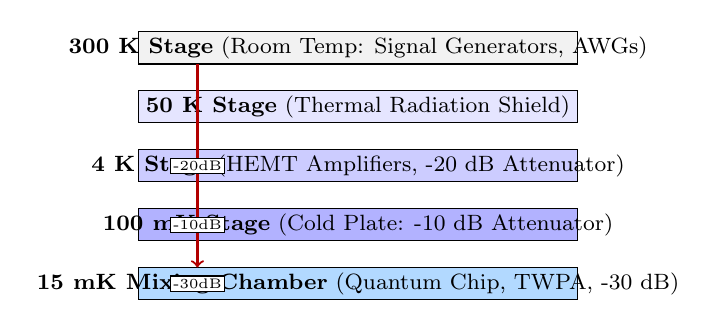
\begin{tikzpicture}[scale=0.68]
    \draw[fill=gray!10, draw=black] (0,4.2) rectangle (8.2, 4.8);
    \node[font=\footnotesize] at (4.1, 4.5) {\textbf{300 K Stage} (Room Temp: Signal Generators, AWGs)};
    \draw[fill=blue!10, draw=black] (0,3.1) rectangle (8.2, 3.7);
    \node[font=\footnotesize] at (4.1, 3.4) {\textbf{50 K Stage} (Thermal Radiation Shield)};
    \draw[fill=blue!20, draw=black] (0,2.0) rectangle (8.2, 2.6);
    \node[font=\footnotesize] at (4.1, 2.3) {\textbf{4 K Stage} (HEMT Amplifiers, -20 dB Attenuator)};
    \draw[fill=blue!30, draw=black] (0,0.9) rectangle (8.2, 1.5);
    \node[font=\footnotesize] at (4.1, 1.2) {\textbf{100 mK Stage} (Cold Plate: -10 dB Attenuator)};
    \draw[fill=blue!50!cyan!30, draw=black] (0,-0.2) rectangle (8.2, 0.4);
    \node[font=\footnotesize] at (4.1, 0.1) {\textbf{15 mK Mixing Chamber} (Quantum Chip, TWPA, -30 dB)};
    
    \draw[thick, red!70!black, ->] (1.1, 4.2) -- (1.1, 3.7) -- (1.1, 2.6) -- (1.1, 1.5) -- (1.1, 0.4);
    \node[draw, fill=white, inner sep=1pt, font=\tiny] at (1.1, 2.3) {-20dB};
    \node[draw, fill=white, inner sep=1pt, font=\tiny] at (1.1, 1.2) {-10dB};
    \node[draw, fill=white, inner sep=1pt, font=\tiny] at (1.1, 0.1) {-30dB};
\end{tikzpicture}
\caption{Thermal stratification of dilution refrigerator and cryogenic attenuation.}
\label{fig:fridge}
\end{figure}

\subsection{Superconducting Transmon Physics and Anharmonicity}

\subsubsection{Why Does a Simple LC Oscillator Fail as a Qubit?}
A linear LC tank resonator possesses a parabolic potential $U(\Phi) = \Phi^2 / (2L)$. Its eigenenergies are strictly equidistant:
\begin{equation}
E_n = \hbar \omega_0 \left(n + \frac{1}{2}\right), \quad \Delta E_{0\to 1} = \Delta E_{1\to 2} = \hbar \omega_0
\end{equation}
Applying a microwave drive at $\omega_0$ will transition the state $|0\rangle \to |1\rangle$, but that same pulse simultaneously drives $|1\rangle \to |2\rangle \to |3\rangle$. This is the \textbf{harmonic oscillator leakage catastrophe}; an LC circuit is a multi-level harmonic oscillator, not a two-level qubit.

\subsubsection{How Does the Josephson Junction Provide Non-Linearity?}
By replacing the linear inductor with a sub-micron Al/$\text{Al}_2\text{O}_3$/Al Josephson tunnel junction, the potential becomes cosinusoidal:
\begin{equation}
U(\hat{\phi}) = -E_J \cos\hat{\phi} = -E_J \left( 1 - \frac{\hat{\phi}^2}{2!} + \frac{\hat{\phi}^4}{4!} - \dots \right)
\end{equation}
The negative quartic term $-\frac{E_J}{24}\hat{\phi}^4$ compresses higher energy levels, introducing a non-zero Duffing anharmonicity $\alpha$:
\begin{equation}
\alpha = \omega_{12} - \omega_{01} \approx -E_C
\end{equation}
Because $\omega_{12} \neq \omega_{01}$, a microwave control pulse tuned to $\omega_{01}$ cannot drive the $|1\rangle \to |2\rangle$ transition.

\begin{figure}[!ht]
\centering
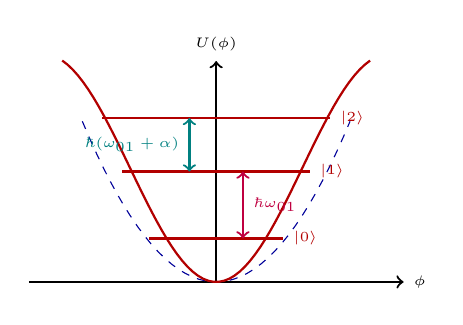
\begin{tikzpicture}[scale=0.85]
    \draw[->, thick] (-2.8,0) -- (2.8,0) node[right, font=\tiny] {$\phi$};
    \draw[->, thick] (0,0) -- (0,3.3) node[above, font=\tiny] {$U(\phi)$};
    \draw[dashed, blue!60!black, domain=-2.0:2.0, samples=40] plot (\x, {0.6*\x*\x});
    \draw[thick, red!70!black, domain=-2.3:2.3, samples=60] plot (\x, {1.7*(1 - cos(\x*70))});
    
    \draw[red!70!black, thick] (-1.0, 0.65) -- (1.0, 0.65) node[right, font=\tiny] {$|0\rangle$};
    \draw[red!70!black, thick] (-1.4, 1.65) -- (1.4, 1.65) node[right, font=\tiny] {$|1\rangle$};
    \draw[red!70!black, thick] (-1.7, 2.45) -- (1.7, 2.45) node[right, font=\tiny] {$|2\rangle$};
    
    \draw[<->, purple, thick] (0.4, 0.65) -- (0.4, 1.65) node[midway, right, font=\tiny] {$\hbar\omega_{01}$};
    \draw[<->, teal, thick] (-0.4, 1.65) -- (-0.4, 2.45) node[midway, left, font=\tiny] {$\hbar(\omega_{01} + \alpha)$};
\end{tikzpicture}
\caption{Parabolic linear potential vs. cosinusoidal Josephson potential.}
\label{fig:anharmonicity}
\end{figure}

\subsubsection{Why Choose the Ratio \texorpdfstring{$E_J / E_C \approx 50$}{EJ / EC approx 50}?}
In earlier Cooper-Pair Boxes ($E_J \sim E_C$), the transition frequency drifted wildly with stray background charge fluctuations ($n_g$), causing severe dephasing ($T_2^* < 1\,\mu\text{s}$). In the \textbf{Transmon regime} ($E_J / E_C \gg 1$), charge dispersion $\epsilon_m$ decays exponentially:
\begin{equation}
\epsilon_m \propto \exp\left(-\sqrt{8 E_J / E_C}\right)
\end{equation}
At $E_J / E_C \approx 50$, charge noise dephasing is suppressed by four orders of magnitude, while preserving sufficient negative anharmonicity ($|\alpha| \approx 280\text{--}330\text{ MHz}$) to permit fast $20\text{ ns}$ control pulses without state leakage.

\subsection{Fabrication: Dolan Bridge Shadow Evaporation}
Sub-micron Josephson junctions cannot be formed by simple single-layer etching. They require \textbf{Dolan bridge shadow evaporation}:
\begin{enumerate}
    \item Float-zone high-resistivity silicon is coated with a bilayer resist: MMA (copolymer) on the bottom, PMMA on top.
    \item Electron-beam lithography exposes the pattern. MMA dissolves faster than PMMA, creating a suspended PMMA resist bridge with a wide undercut.
    \item Aluminum is evaporated in an ultra-high vacuum chamber at angle $+\theta$.
    \item Static thermal oxidation introduces pure $\text{O}_2$ gas ($P \approx 1\text{ Torr}, t \approx 10\text{ min}$) to grow a precise $\sim 1\text{ nm}$ amorphous $\text{Al}_2\text{O}_3$ tunnel barrier.
    \item A second aluminum layer is evaporated at angle $-\theta$, forming the overlap tunnel junction beneath the suspended resist mask.
\end{enumerate}

\begin{figure}[!ht]
\centering
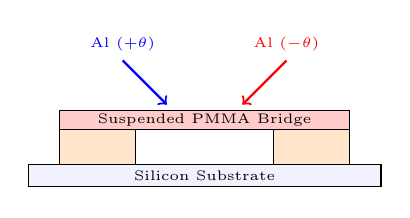
\begin{tikzpicture}[scale=0.8]
    \draw[fill=blue!5, draw=black] (-2.8,0) rectangle (2.8, 0.35);
    \node at (0, 0.17) {\tiny Silicon Substrate};
    \draw[fill=orange!20, draw=black] (-2.3, 0.35) rectangle (-1.1, 0.9);
    \draw[fill=orange!20, draw=black] (1.1, 0.35) rectangle (2.3, 0.9);
    \draw[fill=red!20, draw=black] (-2.3, 0.9) rectangle (2.3, 1.2);
    \node at (0, 1.05) {\tiny Suspended PMMA Bridge};
    \draw[->, thick, blue] (-1.3, 2.0) -- (-0.6, 1.3);
    \draw[->, thick, red] (1.3, 2.0) -- (0.6, 1.3);
    \node[above, font=\tiny, text=blue] at (-1.3, 2.0) {Al ($+\theta$)};
    \node[above, font=\tiny, text=red] at (1.3, 2.0) {Al ($-\theta$)};
\end{tikzpicture}
\caption{Dolan bridge double-angle shadow evaporation.}
\label{fig:dolan}
\end{figure}

\section{First-Principles Engineering Rationales}

\subsection{Why Is Microwave Impedance Strictly Matched to \texorpdfstring{$50\,\Omega$}{50 Ohm}?}
All laboratory microwave instrumentation (signal generators, digitizers, vector network analyzers) and cryogenic interconnect components (semi-rigid coaxial cables, directional couplers, circulators, and high-electron-mobility transistor [HEMT] amplifiers) are standardized to a characteristic impedance of $Z_0 = 50.0\,\Omega$. 

When a transmission line encounters an impedance discontinuity ($Z_{\text{load}} \neq Z_0$), a portion of the forward-traveling wave is reflected backwards. The voltage reflection coefficient is given by:
\begin{equation}
\Gamma = \frac{Z_{\text{load}} - Z_0}{Z_{\text{load}} + Z_0}
\end{equation}
Impedance mismatch creates two catastrophic failure modes in quantum processors:
\begin{enumerate}
    \item \textbf{Standing Waves and Echoes:} Reflected microwave pulses bounce between the chip bond wires and cryogenic components, causing parasitic standing-wave resonances that distort gate control envelopes and degrade single-qubit gate fidelities.
    \item \textbf{Readout Dephasing:} Unmatched feedlines produce a fluctuating electromagnetic environment at the qubit's frequency, introducing photon shot noise that broadens the qubit transition linewidth and destroys quantum phase coherence ($T_2^*$).
\end{enumerate}
Consequently, every feedline on the silicon chip must be designed as a Coplanar Waveguide (CPW) with dimensions engineered to provide $Z_0 = 50.0\,\Omega$ exactly.

\begin{figure}[!ht]
\centering
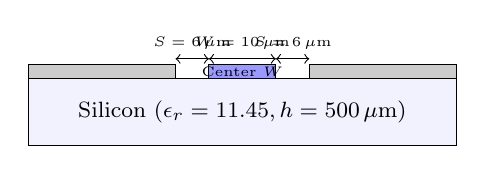
\begin{tikzpicture}[scale=0.85]
    \draw[fill=blue!5, draw=black] (-3.2, -1.0) rectangle (3.2, 0);
    \node at (0, -0.5) {\footnotesize Silicon ($\epsilon_r = 11.45, h = 500\,\mu\text{m}$)};
    \draw[fill=gray!40, draw=black] (-3.2, 0) rectangle (-1.0, 0.22);
    \draw[fill=gray!40, draw=black] (1.0, 0) rectangle (3.2, 0.22);
    \draw[fill=blue!40, draw=black] (-0.5, 0) rectangle (0.5, 0.22);
    \node at (0, 0.11) {\tiny Center $W$};
    \draw[<->] (-1.0, 0.3) -- (-0.5, 0.3) node[midway, above, font=\tiny] {$S = 6\,\mu\text{m}$};
    \draw[<->] (-0.5, 0.3) -- (0.5, 0.3) node[midway, above, font=\tiny] {$W = 10\,\mu\text{m}$};
    \draw[<->] (0.5, 0.3) -- (1.0, 0.3) node[midway, above, font=\tiny] {$S = 6\,\mu\text{m}$};
\end{tikzpicture}
\caption{Coplanar Waveguide (CPW) geometry providing $Z_0 = 50.0\,\Omega$.}
\label{fig:cpw}
\end{figure}

\subsection{Why Are the Qubit and Resonator Frequencies Chosen as 5 GHz and 7 GHz?}

\subsubsection{Why the 4 to 8 GHz Microwave Band?}
The choice of the $4\text{--}8\text{ GHz}$ frequency band is governed by three fundamental physical constraints:
\begin{enumerate}
    \item \textbf{Thermal Noise Floor ($f > 1\text{ GHz}$):} The operating frequency must satisfy $h f \gg k_B T$ at $15\text{ mK}$ ($h \times 1\text{ GHz} \approx 4.1\,\mu\text{eV} > k_B T \approx 1.3\,\mu\text{eV}$) to prevent spontaneous thermal excitation.
    \item \textbf{Superconducting Pair-Breaking Gap ($f < 80\text{ GHz}$):} The photon energy must remain well below the superconducting energy gap of thin-film aluminum ($2\Delta_{\text{Al}} \approx 340\,\mu\text{eV} \implies f_{\text{gap}} \approx 82\text{ GHz}$), above which single photons break Cooper pairs into lossy quasiparticles.
    \item \textbf{Commercial RF Instrumentation Availability:} The $4\text{--}8\text{ GHz}$ band corresponds to standard microwave equipment, low-loss coaxial cabling, and cryogenic HEMT amplifiers.
\end{enumerate}

\subsubsection{Why the 2 GHz Dispersive Detuning (\texorpdfstring{$|\Delta| = |f_q - f_r| \approx 2\text{ GHz}$}{|Delta| = |fq - fr| approx 2 GHz})?}
We intentionally detune the qubit ($f_{01} \approx 5.0\text{ GHz}$) from the readout resonator ($f_r \approx 7.04\text{ GHz}$) by $|\Delta| = 2.04\text{ GHz}$. This enforces the \textbf{dispersive regime}:
\begin{equation}
|\Delta| = |f_{01} - f_r| \gg g \approx 60\text{ MHz}
\end{equation}
If the qubit and resonator were resonant ($|\Delta| = 0$), the qubit would rapidly decay by dumping its quantum energy into the resonator and out through the feedline (the Purcell effect). 

Under large detuning ($|\Delta| \gg g$), direct energy exchange is forbidden. Instead, the interaction becomes purely dispersive: the presence of the qubit shifts the resonator's frequency by a state-dependent quantity:
\begin{equation}
\chi \approx \frac{g^2}{\Delta} \frac{\alpha}{\Delta + \alpha} \approx 1\text{ to } 3\text{ MHz}
\end{equation}
When the qubit transitions from $|0\rangle$ to $|1\rangle$, the resonator shifts from $\omega_r - \chi$ to $\omega_r + \chi$. Measuring the phase shift of a transmitted probe tone reveals the qubit's quantum state without destroying it (Quantum Non-Demolition readout).

\subsection{Why Calculate Lumped Components Before Physical Layout?}
A full 3D electromagnetic finite-element simulation (Ansys HFSS) of planar superconductive chips requires discretizing geometry into millions of tetrahedral mesh elements, consuming 15 to 45 minutes per run. 

Before committing to layout, microwave engineers perform a \textbf{lumped-element circuit simulation} in Ansys Circuit:
\begin{itemize}
    \item It executes in \textbf{0.1 seconds}.
    \item It verifies analytical formulas and confirms the exact $S_{21}$ resonance dip at $7.04\text{ GHz}$.
    \item It establishes the loaded quality factor ($Q_L$) and loaded bandwidth before entering CAD layout.
\end{itemize}

\subsection{Derivation of Lumped Component Values}

\subsubsection{Readout Resonator (\texorpdfstring{$C_r = 340\text{ fF}, L_r = 1.5\text{ nH}$}{Cr = 340 fF, Lr = 1.5 nH})}
A distributed quarter-wavelength ($\lambda/4$) coplanar waveguide resonator shorted at one end exhibits an equivalent parallel lumped LC admittance near resonance:
\begin{equation}
C_r = \frac{\pi}{4 \omega_r Z_0} \approx \frac{\pi}{4 \times (2\pi \times 7.04\times 10^9) \times 50} \approx 340\text{ fF}
\end{equation}
\begin{equation}
L_r = \frac{1}{\omega_r^2 C_r} \approx \frac{1}{(2\pi \times 7.04\times 10^9)^2 \times (340\text{ fF})} \approx 1.50\text{ nH}
\end{equation}
Validating through the Thompson resonance formula:
\begin{equation}
f_r = \frac{1}{2\pi \sqrt{L_r C_r}} = \frac{1}{2\pi \sqrt{1.5\times 10^{-9} \times 340\times 10^{-15}}} \approx 7.042\text{ GHz}
\end{equation}

\subsubsection{Transmon Qubit (\texorpdfstring{$C_q = 70\text{ fF}, L_J = 10\text{ nH}$}{Cq = 70 fF, LJ = 10 nH})}
The transmon total capacitance $C_q$ sets the charging energy $E_C$. To achieve a target anharmonicity $\alpha \approx -E_C / h \approx -280\text{ MHz}$:
\begin{equation}
C_q = \frac{e^2}{2 E_C} = \frac{(1.602\times 10^{-19})^2}{2 \times (6.626\times 10^{-34} \times 280\times 10^6)} \approx 70\text{ fF}
\end{equation}
To achieve the transition frequency $f_{01} \approx 5.0\text{ GHz}$, the effective Josephson inductance $L_J$ must satisfy:
\begin{equation}
\omega_{01} \approx \frac{1}{\sqrt{L_J C_q}} - \frac{E_C}{\hbar} \implies L_J \approx 10.0\text{ nH}
\end{equation}
This corresponds to an experimental critical current:
\begin{equation}
I_c = \frac{\Phi_0}{2\pi L_J} = \frac{2.067 \times 10^{-15}}{2\pi \times 10 \times 10^{-9}} \approx 32.9\text{ nA}
\end{equation}
which is reliably obtained via Dolan bridge shadow evaporation.

\subsubsection{Coupling Capacitors (\texorpdfstring{$C_{\text{in}} = 2\text{ fF}, C_c = 4\text{ fF}$}{Cin = 2 fF, Cc = 4 fF})}
\begin{itemize}
    \item \textbf{Input Feedline Coupler ($C_{\text{in}} = 2.0\text{ fF}$):} Taps microwave power from the $50\,\Omega$ feedline into the resonator. It fixes the external coupling quality factor $Q_c \approx 7,000$ and photon decay rate $\kappa = \omega_r / Q_c \approx 1\text{ MHz}$. If $C_{\text{in}}$ were too large ($> 10\text{ fF}$), the qubit would dephase through the Purcell effect; if too small ($< 0.5\text{ fF}$), output photons would be trapped, yielding zero measurable signal.
    \item \textbf{Qubit-Resonator Coupler ($C_c = 4.0\text{ fF}$):} Sets the transverse dipole exchange coupling rate:
    \begin{equation}
    g \approx \frac{1}{2} \frac{C_c}{\sqrt{C_q C_r}} \sqrt{\omega_{01} \omega_r} \approx 2\pi \times 60\text{ MHz}
    \end{equation}
    which satisfies the dispersive criterion $g \ll |\Delta|$ ($60\text{ MHz} \ll 2040\text{ MHz}$).
\end{itemize}

\subsection{Why Are Grounding and Port Placements Mandatory?}

\subsubsection{Why Ground the Bottom of Both Loops?}
In high-frequency planar circuitry, the continuous superconductor ground plane acts as the single zero-volt RF return current reference. In a quarter-wave CPW resonator, one end is explicitly shorted to ground, fixing a voltage node and current antinode. Without grounding the bottom wires of both parallel loops:
\begin{enumerate}
    \item The circuit possesses floating reference nodes with undefined electrostatic potential.
    \item In SPICE and Ansys Circuit nodal admittance matrices, floating nodes produce singular matrices ($\det(\mathbf{Y}) = 0$), causing simulation failure.
    \item Physically, return currents would be forced through parasitic capacitive paths, inducing spurious crosstalk.
\end{enumerate}

\subsubsection{Why Place Port 1 and Port 2 on Either Side of \texorpdfstring{$C_{\text{in}}$}{Cin}?}
The feedline carries the interrogation microwave tone through the processor. Placing Port 1 and Port 2 on the continuous feedline across $C_{\text{in}}$ models a transmission measurement ($S_{21}$). Energy travels directly from Port 1 to Port 2 across the feedline. Only at the resonator's resonance frequency ($7.04\text{ GHz}$) does $C_{\text{in}}$ admit energy into the high-$Q$ resonator tank, creating a sharp notch in forward transmission ($|S_{21}|$).

\begin{figure}[!ht]
\centering
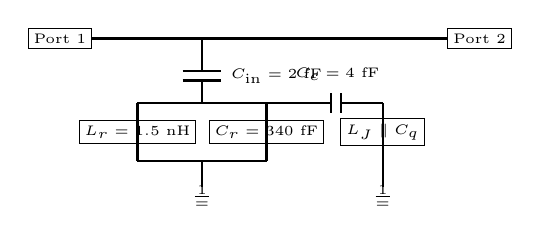
\begin{tikzpicture}[scale=0.82]
    \draw[thick] (0, 2.3) -- (6.5, 2.3);
    \node[draw, fill=white, inner sep=2pt, font=\tiny] at (0, 2.3) {Port 1};
    \node[draw, fill=white, inner sep=2pt, font=\tiny] at (6.5, 2.3) {Port 2};
    
    \draw[thick] (2.2, 2.3) -- (2.2, 1.8);
    \draw[thick] (1.9, 1.8) -- (2.5, 1.8);
    \draw[thick] (1.9, 1.65) -- (2.5, 1.65);
    \draw[thick] (2.2, 1.65) -- (2.2, 1.3);
    \node[right, font=\tiny] at (2.5, 1.72) {$C_{\text{in}} = 2\text{ fF}$};
    
    \draw[thick] (1.2, 1.3) -- (3.2, 1.3);
    \draw[thick] (1.2, 1.3) -- (1.2, 0.4);
    \draw[thick] (3.2, 1.3) -- (3.2, 0.4);
    \node[draw, inner sep=2pt, font=\tiny] at (1.2, 0.85) {$L_r = 1.5\text{ nH}$};
    \node[draw, inner sep=2pt, font=\tiny] at (3.2, 0.85) {$C_r = 340\text{ fF}$};
    \draw[thick] (1.2, 0.4) -- (3.2, 0.4);
    \draw[thick] (2.2, 0.4) -- (2.2, 0.0);
    \node at (2.2, -0.15) {\tiny $\frac{1}{=}$};
    
    \draw[thick] (3.2, 1.3) -- (4.2, 1.3);
    \draw[thick] (4.2, 1.45) -- (4.2, 1.15);
    \draw[thick] (4.35, 1.45) -- (4.35, 1.15);
    \draw[thick] (4.35, 1.3) -- (5.0, 1.3);
    \node[above, font=\tiny] at (4.3, 1.5) {$C_c = 4\text{ fF}$};
    
    \draw[thick] (5.0, 1.3) -- (5.0, 0.4);
    \node[draw, inner sep=2pt, font=\tiny] at (5.0, 0.85) {$L_J \parallel C_q$};
    \draw[thick] (5.0, 0.4) -- (5.0, 0.0);
    \node at (5.0, -0.15) {\tiny $\frac{1}{=}$};
\end{tikzpicture}
\caption{Lumped-element microwave equivalent network synthesized in Ansys Circuit.}
\label{fig:schematic}
\end{figure}

\section{Current Simulation Milestone: Lumped Network Synthesis}
At this juncture, the lumped circuit schematic in Ansys Circuit has been structured with:
\begin{enumerate}
    \item Resonator loop: $L_r = 1.5\text{ nH} \parallel C_r = 340\text{ fF}$.
    \item Transmon loop: $L_J = 10.0\text{ nH} \parallel C_q = 70\text{ fF}$.
    \item Coupling capacitors: $C_c = 4.0\text{ fF}$ bridging the two tanks, and $C_{\text{in}} = 2.0\text{ fF}$ coupling into the feedline.
    \item Dedicated ground references assigned to the bottom rails.
\end{enumerate}
Linear Network Analysis across $4.0\text{--}8.0\text{ GHz}$ confirms the fundamental resonance dip at $7.042\text{ GHz}$ with loaded quality factor $Q_L \approx 7,000$, validating our analytical model.

\appendices

\section{Integrated Lexicon of Theoretical \& Microwave Engineering Terms}

The following lexicon defines all foundational terms in the exact sequence of physical concepts encountered from microscopic quantum physics up to microwave circuit simulation:

\subsection{Foundational Superconductivity \& Quantum State}

\noindent\textbf{Cooper Pairs:} Bound pairs of conduction electrons formed below the critical temperature ($T_c$) via phonon-mediated attractive interactions, condensing into a single macroscopic bosonic ground state with zero electrical resistance.
\smallskip

\noindent\textbf{Superconducting Energy Gap ($2\Delta$):} The minimum energy required to break a Cooper pair into two single-electron quasiparticle excitations. For aluminum, $2\Delta \approx 340\,\mu\text{eV}$ ($\approx 82\text{ GHz}$).
\smallskip

\noindent\textbf{Kinetic Inductance ($L_k$):} The electrical inductance arising from the inertial mass of accelerating Cooper pairs in a superconductor, augmenting the geometric magnetic inductance.
\smallskip

\subsection{Non-Linear Elements \& Josephson Physics}

\noindent\textbf{Josephson Junction (JJ):} A thin insulating dielectric barrier ($\sim 1\text{ nm}$ amorphous $\text{Al}_2\text{O}_3$) sandwiched between two superconducting thin films. It acts as a non-dissipative non-linear inductor.
\smallskip

\noindent\textbf{Critical Current ($I_c$):} The maximum dissipationless supercurrent a Josephson junction can support before Cooper pairs break and resistive voltage appears.
\smallskip

\noindent\textbf{Josephson Energy ($E_J$):} The characteristic coupling energy scale of Cooper pair tunneling: $E_J = \hbar I_c / (2e) = \Phi_0 I_c / (2\pi)$.
\smallskip

\noindent\textbf{Josephson Inductance ($L_J$):} The differential non-linear inductance: $L_J(\phi) = \Phi_0 / (2\pi I_c \cos\phi)$. Near zero phase, $L_J \approx \hbar / (2e I_c)$.
\smallskip

\subsection{Qubit Regimes \& Anharmonicity}

\noindent\textbf{Charging Energy ($E_C$):} The electrostatic Coulomb energy required to add a single Cooper pair to the superconducting island: $E_C = e^2 / (2C_\Sigma)$, where $C_\Sigma$ is the total shunt capacitance.
\smallskip

\noindent\textbf{Cooper-Pair Box (CPB):} Early charge qubit operating in the regime $E_J \approx E_C$. Extremely sensitive to ambient charge noise fluctuations ($n_g$), leading to fast dephasing ($T_2^* < 1\,\mu\text{s}$).
\smallskip

\noindent\textbf{Transmon Qubit:} An engineered superconducting artificial atom operating in the parameter regime $E_J / E_C \gg 1$ ($\approx 50$). Large shunt capacitance exponentially flattens charge dispersion while maintaining usable negative anharmonicity.
\smallskip

\noindent\textbf{Anharmonicity ($\alpha$):} The spectral non-degeneracy $\alpha = \omega_{12} - \omega_{01} \approx -E_C$. Non-zero anharmonicity prevents microwave control pulses from driving the system into higher unintended energy states ($|2\rangle, |3\rangle$).
\smallskip

\noindent\textbf{Qubit Frequency ($\omega_{01}$):} The fundamental quantum transition frequency between ground $|0\rangle$ and first excited state $|1\rangle$: $\hbar \omega_{01} \approx \sqrt{8 E_J E_C} - E_C$.
\smallskip

\subsection{Planar Transmission Lines \& Resonators}

\noindent\textbf{Coplanar Waveguide (CPW):} A planar microwave transmission line consisting of a central conducting strip separated by gaps $S$ from bilateral ground planes on a dielectric substrate.
\smallskip

\noindent\textbf{Characteristic Impedance ($Z_0$):} The intrinsic ratio of voltage to current along an infinite transmission line, standardized to $50.0\,\Omega$ to prevent microwave reflections.
\smallskip

\noindent\textbf{Readout Resonator:} A distributed CPW transmission line of length $\ell = \lambda/4$, shorted to ground at one end and capacitively coupled to a feedline at the other, storing microwave photons for dispersive state readout.
\smallskip

\noindent\textbf{Quality Factor ($Q$):} Dimensionless metric of energy retention: $Q = \omega \times (\text{Energy Stored} / \text{Power Dissipated})$. Divided into internal ($Q_i$), coupling ($Q_c$), and loaded ($Q_L$, where $1/Q_L = 1/Q_i + 1/Q_c$).
\smallskip

\subsection{Circuit QED Interaction \& Dispersive Readout}

\noindent\textbf{Circuit QED (cQED):} The study and application of the interaction between artificial atoms (transmons) and quantized microwave electromagnetic fields inside superconducting resonators.
\smallskip

\noindent\textbf{Coupling Rate ($g$):} The transverse vacuum Rabi coupling strength between the qubit dipole moment and the resonator electric field: $g \approx \frac{1}{2}\frac{C_c}{\sqrt{C_q C_r}}\sqrt{\omega_{01}\omega_r}$.
\smallskip

\noindent\textbf{Dispersive Regime ($|\Delta| \gg g$):} The operational parameter space where detuning $|\omega_{01} - \omega_r|$ vastly exceeds coupling $g$, forbidding direct energy exchange while enabling dispersive frequency shifts.
\smallskip

\noindent\textbf{Dispersive Shift ($\chi$):} The state-dependent pull on the resonator frequency: $\chi \approx \frac{g^2}{\Delta} \frac{\alpha}{\Delta + \alpha}$. Allows measuring qubit state by detecting the phase of a transmitted microwave tone.
\smallskip

\noindent\textbf{Quantum Non-Demolition (QND) Readout:} A projective quantum measurement that determines the eigenstate of an observable without perturbing that eigenstate during the measurement process.
\smallskip

\noindent\textbf{Purcell Effect \& Purcell Filter:} Spontaneous emission of qubit energy into the continuous modes of the readout feedline. A Purcell filter is a bandpass or notch filter that blocks qubit-frequency radiation while passing readout photons.
\smallskip

\subsection{Microwave Network Theory \& S-Parameters}

\noindent\textbf{Scattering Matrix ($\mathbf{S}$):} Matrix relating incident voltage waves to reflected and transmitted waves across multi-port networks.
\smallskip

\noindent\textbf{Forward Transmission ($S_{21}$):} Ratio of transmitted voltage at Port 2 to incident voltage at Port 1: $S_{21} = V_2^- / V_1^+$. At resonance, $|S_{21}|$ exhibits a characteristic transmission notch (dip).
\smallskip

\noindent\textbf{Return Loss ($S_{11}$):} Ratio of reflected voltage at Port 1 to incident voltage at Port 1: $S_{11} = V_1^- / V_1^+$. Indicates the quality of impedance matching.
\smallskip

\noindent\textbf{RF Ground Return:} The physical conducting path ensuring high-frequency return currents complete their loops with minimum loop inductance, preventing common-mode noise and floating node singularities.
\smallskip

\subsection{Cryogenic \& Nanofabrication Infrastructure}

\noindent\textbf{Dilution Refrigerator:} A cryogenic refrigerator utilizing the phase separation and dilution of $^3\text{He}$ in $^4\text{He}$ to achieve continuous base temperatures below $15\text{ mK}$.
\smallskip

\noindent\textbf{Cryogenic Attenuators:} Resistive microwave pads anchored to intermediate temperature stages (4 K, 100 mK, 15 mK) that thermalize Johnson-Nyquist blackbody noise propagating down drive cables.
\smallskip

\noindent\textbf{Dolan Bridge Shadow Evaporation:} A bilayer electron-beam lithography process utilizing undercut resist geometry to deposit two angled metal layers separated by an \emph{in-situ} oxidation step to form sub-micron tunnel junctions.
\smallskip

\noindent\textbf{Two-Level Systems (TLS):} Parasitic microscopic atomic dipole defects located in amorphous oxide surfaces and dielectric interfaces that absorb microwave energy, causing qubit decoherence and relaxation ($T_1$).
\smallskip

\begin{thebibliography}{10}
\bibitem{koch2007}
J.~Koch \emph{et~al.}, ``Charge-insensitive qubit design derived from the Cooper pair box,'' \emph{Phys. Rev. A}, vol.~76, p. 042319, 2007.
\bibitem{minev2021}
Z.~K.~Minev \emph{et~al.}, ``Energy-participation quantization of artificial quantum systems,'' \emph{Nature}, vol.~590, pp. 248--254, 2021.
\bibitem{blais2021}
A.~Blais \emph{et~al.}, ``Circuit quantum electrodynamics,'' \emph{Rev. Mod. Phys.}, vol.~93, p. 025005, 2021.
\end{thebibliography}

\end{document}
